\section{\xxx Overview} \label{sec:overview}

\xxx is deployed as a typical \smr system. A set of three or five replicas is 
set up within a LAN, and each replica runs an \xxx instance containing the 
same server program. On the \xxx system starts, one replica becomes the 
\emph{primary} (or leader) replica which proposes the order of requests to 
execute, and the others become backup replicas which follow the primary's 
proposals. A number of clients in LAN or WAN send network requests 
to the primary and get responses.  If the primary machine fails, the other 
replicas run a leader election~\cite{paxos:practical} to elect a new primary.

This section first presents \xxx's architecture, including its consensus 
interface and a \xxx instance's main components, and then uses an 
example to show how \xxx works with server programs.

% \subsection{Usage} \label{sec:usage}
% TBD.

\subsection{Architecture} \label{sec:abstraction}

To support general server programs transparently, \xxx chooses the POSIX socket 
API as its consensus interface. \xxx enforces two kinds of orders for socket
calls. First, for client programs' out going socket calls (\eg, \connect and
\send), \xxx enforces that all replicas see the same sequence of client socket 
calls with \paxos. \xxx does not need to order the clients' 
blocking socket calls because \xxx is not designed to replicate clients. 
Second, for a server program's blocking socket calls (\eg, \poll, \accept, and 
\recv), \xxx enforces that these calls are scheduled and 
returned in the same sequence of logical times across replicas. \xxx 
responses to the clients only using the server program on the primary, and it 
drops the responses of the server programs on backups.

For a server program's outgoing socket calls (\eg, \send), \xxx simply 
schedules them using \dmt and does not invoke consensus. The 
reason is that these calls readily have consistent contents via enforcing 
the same logical admission times of input requests and the same thread 
schedules for server programs across replicas.

\begin{figure}[t]
\centering
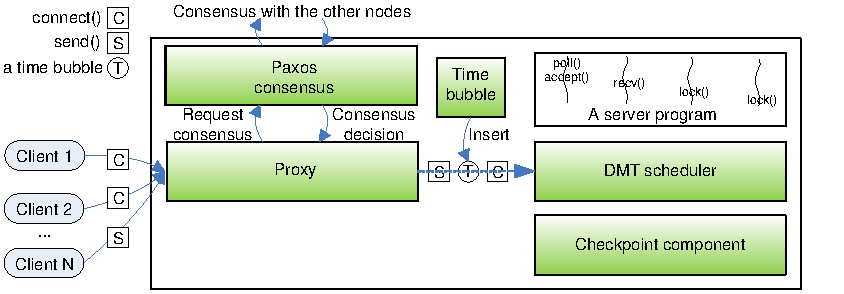
\includegraphics[width=.5\textwidth]{figures/repbox}
% \vspace{-.20in}
\caption{{\em The \xxx Architecture.} \xxx components are shaded (and in
  green).} \label{fig:repbox}
\vspace{-.05in}
\end{figure}

Figure~\ref{fig:repbox} shows a \xxx instance running on the primary. The 
instance contains five main components, the proxy, the 
\paxos consensus, the \dmt scheduler, the \timealgo component that enforces the 
same logical clocks for servers' blocking socket calls across
replicas via inserting time bubbles, and the checkpoint component that 
periodically checkpoints the server program. A server program runs 
transparently in a \xxx instance without being aware of \xxx's components. A 
backup replica runs the same \xxx instance except that its proxy does not 
accept connections from clients and does not invoke consensus.

%% Each component.
The proxy component is a \xxx instance's gateway.  It accepts socket
requests from clients and forwards the requests to the server program on its 
own replica. It accepts responses from the server program and forwards the 
responses to the clients. Once the proxy receives a
client socket request, it invokes the \paxos consensus component running
on its own replica for this request.  The proxy does not block-wait for 
this decision which may take a while to reach. Once the proxy is notified by 
the \paxos component that some requests' decisions are made, it forwards the 
requests in decision order to the server program.

% Only the primary's proxy receives requests from the clients and initiates the 
% consensus process, but every proxy forwards requests to the server program on 
% its own replica.

The \paxos consensus component is a \paxos protocol that receives a client 
socket request from its own proxy and invokes a consensus process on
this request.  This component is also the only \xxx component that
communicates among different replicas. \xxx's \paxos implementation is 
based on a well-known and concise protocol~\cite{paxos:practical}. After
\xxx's \paxos components reach consensus on a client socket call, each \paxos 
component notifies its own proxy to forward this call to its server program.

The \dmt component runs within the server program's process. \xxx leverages 
\parrot~\cite{parrot:sosp13} as the \dmt scheduler because \parrot 
runs fast on a wide range of 108 popular multithreaded programs. Specifically, 
\parrot uses a runtime technique called \ldpreload to dynamically intercept 
\pthread synchronizations (\eg, \mutexlock) issued by an executable and 
enforces a well-define, round-robin schedule on these synchronization 
operations for all threads, practically eliminating nondeterminism in thread 
synchronizations.

Although \parrot is not designed to resolve data races
deterministically, \xxx's replication tolerates data races that have
fail-stop consequences, and can further catch the
other data races by running a race detector on a backup replica (see
\S\ref{sec:limit}).  \xxx augments the \dmt component to schedule the
return points of socket calls in server replicas, too, to ensure that
requests are admitted at consistent logical times across replicas.

The \timealgo component sits between the proxy and the \dmt's processes, and it 
is invoked on two conditions. First, on a server's bootstraps, \xxx invokes 
time bubble insertions to make sure that the server programs across replicas 
reach the same initial state and wait for the first input request. Second, if 
the \dmt component has not received any input request from the proxy for a 
physical duration \ntimeout, a time bubble insertion is invoked as the boundary 
of two request bursts. To ensure the same sequence of inserted time bubbles 
across replicas, the same \paxos consensus as that for client socket calls is 
invoked. For each time bubble, each replica's \dmt scheduler promises to run a 
number of \nclock synchronizations and not to admit any 
client socket call.

If the \dmt scheduler exhausts the logical clocks in a time bubble, it either 
admits new client socket call (if any) or inserts another time bubble. If the 
scheduler does not exhaust the logical clocks after serving current requests, 
\parrot has a mechanism to exhaust them rapidly. More discussions on the values 
of the two parameters \ntimeout and \nclock are given in 
\S\ref{sec:sensitivity}.

% Across different runs of the \xxx system, this physical 
% duration may cause different number of inserted time bubbles; within the same 
% run, \xxx uses \paxos to preserve the same number of inserted time bubbles 
% across different replicas.



To recover from replica failures or add new replicas, the checkpoint 
component is invoked every minute on a backup replica. It
checkpoints the server process running with \dmt.  While one can always start a 
server replica from scratch and replay the entire sequence of socket calls, 
this replay can be extremely time-consuming for long-running servers.  Prior 
\smr systems rely on narrow state machine interfaces for checkpoint and
recovery, which does not work for general server programs. Instead, \xxx
leverages two popular open source tools: \criu, to checkpoint process 
state such as CPU registers and memory; and \lxc, to checkpoint the file 
system state of a server program's current working directory and installation 
directory.

Each checkpoint in \xxx is associated with a global index in \paxos's consensus 
order, so if one replica needs recovery, \xxx ships the latest checkpoint from a 
backup replica, restores the process running \dmt and the server program, and 
re-executes socket calls starting from this index. The proxy and consensus 
components do not require checkpoints because we explicitly designed their 
execution states independent to the server's process.

% \subsection{Building DMT Systems} \label{sec:dmt}
% 
% TBD.

\subsection{Assumptions} \label{sec:limit}

% \xxx's key benefit is that a server program's blocking socket operations and 
% \pthread synchronization operations return at the same logical clocks across 
% different replicas, if a server program has no data race, no ad-hoc 
% synchronization, and does not have nondeterministic functions (\eg, 
% \v{rand()}).

\xxx leverages \parrot to make synchronizations deterministic.  \parrot is
explicitly designed not to handle data races. However, in the context of \xxx,
data races are less harmful because, if they cause backups to crash, \xxx
can still operate and recover as long as a quorum of the replicas is
still alive. Moreover, leveraging \xxx's replication architecture, one can 
deploy a race detector on a backup replica~\cite{repframe:apsys15}, achieving 
both good \xxx performance and full determinism.

There are other sources of nondeterminism besides thread scheduling and
request timing.  These other sources of nondeterminism may cause backups
to diverge, too.  For example, backups may do different things based on
their IP addresses, data read from \v{/dev/random}, addresses returned by
\v{malloc}, physical time observed via \v{gettimeofday}, or delivery time
of signals.  Prior work has shown how to eliminate these sources of
nondeterminism using record-replay~\cite{scribe:sigmetrics2010, 
respec:asplos10} or OS-level techniques~\cite{dos:osdi10}, which \xxx can 
leverage.  Another solution is to treat all these sources as inputs and 
leverage distributed consensus to let all replicas observe the same input.  We 
leave these ideas for future work. We inspected server 
programs' network outputs among replicas, and we found that these outputs 
were consistent in \xxx except physical times (\S\ref{sec:correctness}).

For a server program that spawns multiple processes which communicate via
IPC, \xxx currently does not make these IPC operations deterministic.  We
expect that it should be easy to support deterministic IPC in \xxx because it
already makes socket API deterministic.  In addition,
dOS~\cite{dos:osdi10} and DDOS~\cite{ddos:asplos13} have many effective
techniques for tackling this problem, which \xxx can leverage.

%% Overall guarantee. But go high level.

% 
% \subsection{Example} \label{sec:example}
% 
% \begin{figure}[t]
% \centering
% \begin{minipage}{.5\textwidth}
% \lgrindfile{code/example.cpp.lineno}
% \end{minipage}
% \vspace{-.1in}
% \caption{{\em A server example based on \apache.}} \label{fig:example}
% \vspace{-.20in}
% \end{figure}
% 
% \begin{figure}[t]
% \centering
% \begin{minipage}{.5\textwidth}
% \lgrindfile{code/client.cpp.lineno}
% \end{minipage}
% \vspace{-.1in}
% \caption{{\em A client example based on \v{curl}.}} \label{fig:client}
% \vspace{-.05in}
% \end{figure}
% 
% %TBD. Overall intro on the code.
% Figure~\ref{fig:example} shows an example based on the \apache \http server. For 
% clarity, the example uses worklist synchronization, and the actual servers use 
% \pthread mutex locks and conditional variables which \xxx readily handles. The 
% main thread creates a listener thread to accept client requests and a number 
% of worker threads to process client requests in parallel. The listener listens 
% on a port with \poll. When a new client connection comes, the 
% listener calls \accept and appends the accepted socket descriptor to a 
% worklist. Each worker thread blocks on a \v{worklist.get()} function until 
% the worklist is not empty. It then dequeues an accepted socket, processes the 
% request with a mutex lock acquired, and then sends a response. 
% Figure~\ref{fig:client} shows an example based on client programs such as 
% \v{curl}. This client connects to the server, sends one \http request, waits for 
% the server's response, and then closes the connection.
% 
% Let's say a \xxx system with three replicas is set up, and each replica runs 
% this server; two clients start simultaneously, and each sends a \http PUT 
% and GET request respectively on the same URL ``a.php" to the primary.
% 
% 
% 
% \begin{figure}[t]
% \centering
% \begin{minipage}{.5\textwidth}
% \lgrindfile{code/diff-sync-order.cpp}
% \end{minipage}
% \vspace{-.1in}
% \caption{{\em HTTP GET request got the valid page due to the two requests' 
% large arrival interval.}} \label{fig:yes-page}
% \vspace{-.2in}
% \end{figure}
% 
% \begin{figure}[t]
% \centering
% \begin{minipage}{.5\textwidth}
% \lgrindfile{code/diff2-sync-order.cpp}
% \end{minipage}
% \vspace{-.1in}
% \caption{{\em HTTP GET request didn't get the page due to the two requests'
% small arrival interval.}} \label{fig:no-page}
% \vspace{-.05in}
% \end{figure}
% 
% 
% % If for example
% % there are multiple such clients sending POST requests simultaneously, the
% % order in which the requests are processed can lead to different server
% % states.
% 
% This server has three major sources of nondeterminism, 
% which can easily cause its execution states across 
% replicas to diverge. The first source (for short, $S_1$) is that clients' 
% requests may arrive at different replicas in different orders. Second ($S_2$), 
% within the server, the nondeterministic \pthread synchronizations may easily 
% lead to different schedules. For instance, the \v{worklist.add()} called by 
% the listener may wake up any worker blocking on \v{worklist.get()}.
% 
% Third ($S_3$), even if clients' requests arrive at different replicas in the 
% same order, the physical time interval of each two consecutive requests can 
% still be largely different across replicas depending on each request's physical 
% arrival time. This variance may cause client socket calls to be 
% admitted at inconsistent logical clocks across replica and lead to divergent 
% execution states.
% 
% For instance, Figure~\ref{fig:yes-page} and Figure~\ref{fig:no-page} show two 
% replicas' schedules, and each is a total order of executed socket calls or 
% \pthread synchronizations in workers. Although the PUT and 
% GET requests arrive at the two replicas in the same order, these requests' 
% interval in the first schedule (Figure~\ref{fig:yes-page}) is much larger than 
% that in the second one, causing the first one to return a page and the second 
% one ``404 Not Found".
% 
% % even one 
% % can always enforce that the PUT request arrives before the GET request, because 
% % worker 2's \recv call in Figure~\ref{fig:yes-page} returns much later than that 
% % in Figure~\ref{fig:no-page} (the line numbers in these figures can be viewed as 
% % logical times), two different schedules and thus different outputs may show up.
% 
% % Worse, 
% % the workers' \v{process\_req()} functions contain extra \pthread 
% % synchronizations, then the server's blocking socket operations can return at 
% % arbitrary logical points which interleave nondeterministically with these 
% % synchronizations, easily leading to different schedules and execution states 
% % across machines.
% 
% \begin{figure}[t]
% \centering
% \lgrindfile{code/paxos-queue-order.cpp}
% \vspace{-.2in}
% \caption{{\em A sequence of client socket calls enforced by 
% \xxx.}}\label{fig:paxos-queue}
% \vspace{-.25in}
% \end{figure}
% 
% \begin{figure}[t]
% \centering
% \lgrindfile{code/example-sync-order.cpp}
% \vspace{-.2in}
% \caption{{\em A schedule of the server example enforced by 
% \xxx across replicas.}}\label{fig:dmt-schedule}
% \vspace{-.05in}
% \end{figure}
% 
% 
% \xxx works as follows. First, depending on the order the primary's proxy 
% receives these requests, \xxx eliminates $S_1$ with \paxos and ensures the 
% same request sequence for all replicas. Second, \xxx's \dmt 
% scheduler eliminates $S_2$ by ensuring a deterministic order of \pthread 
% synchronizations.
% 
% Third, depending on the time intervals of client socket calls 
% observed by the primary, \xxx eliminates $S_3$ by dividing this sequence of 
% calls into bursts with time bubbles. Figure~\ref{fig:paxos-queue} shows a 
% sequence. Let's say the primary observes that the 
% intervals of the \connect and \send calls are all smaller than \ntimeout, and 
% the interval between the \send at Line 4 and the \close at Line 6 in the 
% sequence is larger than \ntimeout. Then, \xxx inserts a time bubble at Line 5 
% and divides the sequence into two bursts. For the calls in the first burst, all 
% replicas admit them as is using \dmt even if some of their time intervals are 
% larger than \ntimeout on some backups, consistently maintaining the logical 
% admission times for these calls.
% 
% For the time bubble in this sequence, all replicas' \dmt schedulers promise to 
% do only \nclock \pthread synchronizations and then admit a client 
% socket call, consistently maintaining the logical admission times 
% for the \close calls. Given this sequence, Figure~\ref{fig:dmt-schedule} shows 
% \xxx's consistent schedule and output ``404 Not Found" across replicas. 
% We ran \xxx with \apache and used \v{curl} to spawn concurrent PUT 
% and GET requests, and we observed that \apache's network outputs were 
% consistent across replicas (\S\ref{sec:correctness}).
% 
% In addition to enforcing consistency, the \timealgo technique is 
% also efficient because it does per-burst consensus instead of per-request 
% consensus. In this example, if more \connect calls arrive simultaneously and 
% each client connection does more \send calls, the ratio of inserted 
% time bubbles versus the total number of socket calls in the sequence may be 
% even lower, then \xxx may become more efficient. Evaluation on popular servers 
% and workloads shows that this ratio is often low and that \xxx has moderate 
% overhead  (\S\ref{sec:overhead}).

% according to the primary's physical duration check on 
% \ntimeout, \xxx eliminates $S_3$ by inserting time bubbles which divide the 
% client requests into bursts. For the socket calls within each burst, \xxx's \dmt 
% schedulers consistently admit these calls as is regardless of the differences of 
% each call's physical arrival times across replicas. For each time bubble, \xxx's 
% \dmt schedulers across replicas promise to tick \nclock \pthread 
% synchronizations and not to admit any client socket call before then.



% KEY: Explain why there is such order fo client requests, and why there must be 
% A timebubble. Also explain the 100us boundary. Also, justified by experiments. 
% Also explain subsequent timebubbles may also be inserted.


% Enforcing logical admission times across replicas for the these socket calls 
% consistently is challenging. Consider the \close calls, on 
% the client side, the clients won't execute \close until the server sends 
% responses. On the server side, the server's worker threads keep executing 
% \pthread synchronizations and ticking \dmt's logical clocks. From a \dmt 
% scheduler's view, the clients' \close are external inputs and may be appended 
% to each replica's sequence at indefinite physical times. Therefore, these calls 
% and further socket calls may be admitted by the \dmt schedulers across 
% replicas at inconsistent logical clocks.

% In short, \xxx must ensure that these 
% \close calls are admitted by the \dmt schedulers across replicas at consistent 
% logical times.

% To tackle this challenge, \xxx inserts a time bubble at Line 5 of the sequence 
% to divide the client socket calls into two bursts. For each time bubble, the 
% \dmt scheduler promises to schedule exactly \nclock thread synchronizations and 
% not to admit any client socket call before then. If the server needs to execute 
% more \pthread synchronizations to process requests so that responses can be 
% sent and clients' \close calls can come, \xxx inserts more time bubbles. If 
% there are leftover clocks in a time bubble, \parrot, \xxx's \dmt scheduler, has 
% a mechanism to exhaust these clocks rapidly (\S\ref{sec:parrot}).

% KEY: explain why we did not need a time bubble for each request.
% In addition to addressing the consistency challenge, the \timealgo technique is 
% also efficient because it does per-burst consensus instead of per-request 
% consensus. From this example we can see that per-request consensus is 
% unnecessary because once the server's \accept calls return, the clients can do 
% \send calls immediately, making clients' \connect and \send come in one burst. 
% If more client \connect calls come simultaneously and each connection does more 
% \send calls, the ratio of inserted time bubbles vesus the total number of 
% socket calls in the sequence may be even lower, then \xxx may become more 
% efficient. Evaluation on popular servers and workloads confirmed that 
% this ratio is often low (\S\ref{sec:overhead}).


% KEY: change description: since incoming sequence is ready, timebubbles are 
% ready, so \dmt just schedules them as is. Three types of operations: regular 
% sync, blocking socket calls, and outgoing socket calls. Third, 
% Figure~\ref{fig:schedule}. 
% Given the sequence in Figure~\ref{fig:paxos-queue}, the \dmt scheduler's task 
% becomes easy. It pops the first client socket call in the sequence and 
% schedules a server thread blocking on a matching socket call. 
% For instance, \dmt schedules a server thread blocking on a \recv with a 
% matching \send in the sequence. If the \dmt scheduler sees a time bubble at 
% sequence head, it decreases this bubble's logical clock by one and does a 
% \pthread synchronization or a outgoing socket call (\eg, \send in Line 22 in 
% Figure~\ref{fig:example}). When the time bubble has no clock left, \dmt pops it 
% and postpones to schedule any synchronization until the next time bubble or 
% client socket call comes. If the primary's \dmt scheduler sees no client socket 
% call comes after postponing for a physical duration \ntimeout, it invokes a 
% \paxos consensus on ``inserting a time bubble" (\S\ref{sec:time-bubble}). 



% Let's say \xxx's primary sees that the \connect and \send calls 
% come in almost the same physical time, and it sees that the \close calls 
% come after the \send calls later than the physical duration \ntimeout.
% Figure~\ref{fig:paxos-queue} shows a sequence of the two 
% clients' outgoing socket calls and a time bubble inserted by \xxx. Because the 
% primary sees that the two \send calls come closely, it groups 
% these calls within the same burst. Then, even if the second \send call reaches 
% the other backups much later than the first \send call, \xxx consistently 
% treats the two \send calls as one burst across replicas. To match these two 
% \send calls, \xxx schedules the two \recv calls one next to the other at Line 9 
% and 10 in Figure~\ref{fig:dmt-schedule}, ensuring consistent logical clocks for 
% these \recv calls across replicas.
% 
% In addition, because the primary inserts a time bubble at Line 5 in 
% Figure~\ref{fig:paxos-queue}, all replicas consistently handle this time bubble 
% by ticking \nclock logical clocks and then admit the two \close calls, ensuring 
% consistent logical clocks for these two \close calls across replicas. 




% However, in real-world, the clients' socket operations do not come in one
% single burst. The reasons can be network congestion causing a delay, or
% the clients just waiting for the server's responses.  For example, our
% client program waits for a response from the server before it closes the
% connections.  When the \paxos socket request queue is empty and one of the
% threads wants to do a blocking network operation, the \dmt component
% cannot just block the thread and let other threads run until the next
% request arrives.  If it does so, the next request will most likely be
% admitted at different logical times across replicas because replicas run
% and advance their logical times at different speeds.  The \dmt component
% cannot just block all threads, either, because there are requests being
% processed and the next request may lag indefinitely.  

% To address this timing issue, we have created a new technique called
% \timealgo.  The \dmt scheduler waits for a short amount of time, and if
% the queue is still empty, \dmt requests the proxy to insert a time bubble
% to the queue which contains a fixed amount of logical clocks. The primary
% node's proxy asks for consensus on a time bubble insertion into the \paxos
% queue. After replicas reach consensus on this insertion, each machine's
% \dmt scheduler can tick the same amount of logical clocks in this time
% bubble to process already admitted requests and send responses to
% clients. More time bubbles will be inserted if necessary. If there are
% leftover clocks in a time bubble, when new requests come, the \dmt
% scheduler \xxx leverages invokes an \emph{idle thread} mechanism
% (\S~\ref{sec:parrot}) to quickly consume these clocks consistently across
% machines and process new requests.

% Figure~\ref{fig:paxos-queue} shows a sequence of client socket operations with 
% a time bubble \xxx inserts. By enforcing this same sequence across different 
% machines, \xxx enforces the same sequence of logical clocks and thus the same 
% resultant schedules across different machines, as shown in 
% Figure~\ref{fig:dmt-schedule}.

 


% When the primary fails and a new primary is elected, clients need a way to
% connect to the new primary or transparently migrate their existing
% connections to the new primary.  We assume some standard fail-over
% DNS/networking techniques in place for this purpose as in existing
% replication systems.
